\section{Equivalence of Models}\label{sec:equivalenceofmodelsregular}

\firstwords{By now, we've learned} about a handful of different models of computation: regular expressions, deterministic finite automata, nondeterministic finite automata, and nondeterministic finite automata with epsilon transitions. Regular expressions give us a textual, language-oriented way of reasoning about regular languages, while finite automata allow us to think graphically in terms of machines. While these two approaches may seem far apart, there actually isn't as much difference between them as one might think.

Let's focus on finite automata for a moment. Going from deterministic to nondeterministic models, we saw that we can construct finite automata that both recognize the same language and are easier to understand---for instance, by virtue of having fewer states or transitions. By introducing epsilon transitions, we learned that we don't even necessarily need to read symbols in order to transition from one state to another.

It seems that this ongoing weakening of conditions keeps giving us models that can ``do more". You may be surprised to learn, however, that all of these models of computation are equivalent in terms of the languages they can recognize! No matter what flavour of finite automaton we have, we don't actually gain any additional recognition power.

We will prove this automaton equivalence in two steps. First, we will devise a procedure to convert from a nondeterministic finite automaton with epsilon transitions to one without. Afterward, we will see how to convert from a nondeterministic finite automaton to a deterministic finite automaton.

\subsection{$\ENFA = \NFA$}

In our first procedure, we will use the notion of \emph{epsilon closure} to remove epsilon transitions from a nondeterministic finite automaton. The epsilon closure of a state $q$ is the set of states where there exists some sequence of epsilon transitions from $q$ to that state. Note that the epsilon closure of $q$ always includes $q$ itself.

\begin{theorem}\label{thm:NFAepsilontoNFA}
Given a nondeterministic finite automaton with epsilon transitions $\mathcal{M}$, we can convert it to a nondeterministic finite automaton $\mathcal{M}'$ without epsilon transitions.

\begin{proof}
Let $\mathcal{M} = (Q, \Sigma, \delta, q_{0}, F)$ be a nondeterministic finite automaton with epsilon transitions. We will construct an equivalent nondeterministic finite automaton $\mathcal{M}' = (Q', \Sigma, \delta', q'_{0}, F')$ without epsilon transitions in the following way:
\begin{enumerate}
\item Take $Q'$ to be the original state set $Q$, and remove all states having only epsilon transitions \emph{to} that state. The initial state is not removed, so take $q'_{0} = q_{0}$. All final states in $\mathcal{M}$ remain final states in $\mathcal{M}'$ unless they were removed.
\item Take $\delta'$ to be the original transition function $\delta$, but with all epsilon transitions removed. For all states removed in the previous step, also remove all transitions \emph{from} that state.
\item Add new transitions to the transition function $\delta'$ as follows:
	\begin{itemize}
	\item If there exists a ``chain" of transitions in $\mathcal{M}$ beginning at a state $q_{i}$ and ending at a state $q_{j}$, where all but the last transition is an epsilon transition and the last transition is on some symbol $a \in \Sigma$,
\begin{center}
\begin{tikzpicture}[node distance=1.5cm, >=latex, every state/.style={fill=white}]
\node[state, inner sep=1pt, minimum size=1.5em] (q0) {$q_{i}$};
\node[state, inner sep=1pt, minimum size=1.5em] (q1) [right of=q0] {};
\node[state, inner sep=1pt, minimum size=1.5em] (q2) [right of=q1, draw=none, fill=none] {$\dots$};
\node[state, inner sep=1pt, minimum size=1.5em] (q3) [right of=q2] {};
\node[state, inner sep=1pt, minimum size=1.5em] (q4) [right of=q3] {$q_{j}$};

\path[-latex] (q0) edge [above] node {$\epsilon$} (q1);
\path[-latex] (q1) edge [above] node {$\epsilon$} (q2);
\path[-latex] (q2) edge [above] node {$\epsilon$} (q3);
\path[-latex] (q3) edge [above] node {$a$} (q4);
\end{tikzpicture}
\end{center}
	then replace this ``chain" in $\mathcal{M}'$ with a single transition on $a$ between $q_{i}$ and $q_{j}$.
\begin{center}
\begin{tikzpicture}[node distance=1.5cm, >=latex, every state/.style={fill=white}]
\node[state, inner sep=1pt, minimum size=1.5em] (q0) {$q_{i}$};
\node[state, inner sep=1pt, minimum size=1.5em] (q1) [right of=q0] {$q_{j}$};

\path[-latex] (q0) edge [above] node {$a$} (q1);
\end{tikzpicture}
\end{center}
	\item If there exists a ``chain" of epsilon transitions in $\mathcal{M}$ beginning at a state $q_{i}$ and ending at a final state $q_{f} \in F$,
\begin{center}
\begin{tikzpicture}[node distance=1.5cm, >=latex, every state/.style={fill=white}]
\node[state, inner sep=1pt, minimum size=1.5em] (q0) {$q_{i}$};
\node[state, inner sep=1pt, minimum size=1.5em] (q1) [right of=q0] {};
\node[state, inner sep=1pt, minimum size=1.5em] (q2) [right of=q1, draw=none, fill=none] {$\dots$};
\node[state, inner sep=1pt, minimum size=1.5em] (q3) [right of=q2] {};
\node[state, accepting, inner sep=1pt, minimum size=1.5em] (q4) [right of=q3] {$q_{f}$};

\path[-latex] (q0) edge [above] node {$\epsilon$} (q1);
\path[-latex] (q1) edge [above] node {$\epsilon$} (q2);
\path[-latex] (q2) edge [above] node {$\epsilon$} (q3);
\path[-latex] (q3) edge [above] node {$\epsilon$} (q4);
\end{tikzpicture}
\end{center}
	then remove this ``chain" from $\mathcal{M}'$ and make $q_{i}$ a final state.
\begin{center}
\begin{tikzpicture}[node distance=1.5cm, >=latex, every state/.style={fill=white}]
\node[state, accepting, inner sep=1pt, minimum size=1.5em] (q0) {$q_{i}$};
\end{tikzpicture}
\end{center}
	\end{itemize}
\end{enumerate}
In this way, we have constructed a nondeterministic finite automaton without epsilon transitions recognizing the same language as the original finite automaton.
\end{proof}
\end{theorem}

\begin{example}
Consider the following nondeterministic finite automaton with epsilon transitions highlighted:
\begin{center}
\begin{tikzpicture}[node distance=2cm, >=latex, every state/.style={fill=white}]
\node[state, initial] (q0) {$q_{0}$};
\node[state, accepting] (q1) [right of=q0] {$q_{1}$};
\node[state] (q2) [right of=q1] {$q_{2}$};

\path[-latex] (q0) edge [loop above] node {$d$} (q0);
\path[-latex] (q0) edge [bend right, below] node {$c$} (q1);
\path[-latex, thick, color=\thirdcolour] (q1) edge [bend right, above] node {$\epsilon$} (q0);
\path[-latex] (q1) edge [loop above] node {$b$} (q1);
\path[-latex] (q1) edge [bend right, below] node {$a$} (q2);
\path[-latex, thick, color=\thirdcolour] (q2) edge [bend right, above] node {$\epsilon$} (q1);
\path[-latex] (q2) edge [loop above] node {$b$} (q2);
\end{tikzpicture}
\end{center}
We will use our construction to convert this to a nondeterministic finite automaton without epsilon transitions.
\begin{enumerate}
\item First, we take our state set $Q'$ and our initial state $q'_{0}$. Since there are no states in this finite automaton having \emph{only} incoming epsilon transitions, we don't need to remove any states.
\begin{center}
\begin{tikzpicture}[node distance=2cm, >=latex, every state/.style={fill=white}]
\node[state, initial] (q0) {$q_{0}$};
\node[state, accepting] (q1) [right of=q0] {$q_{1}$};
\node[state] (q2) [right of=q1] {$q_{2}$};
\end{tikzpicture}
\end{center}
\item Next, we take our transition function $\delta'$ with all epsilon transitions removed. We don't need to remove any other transitions from removed states, since we had no such states in the previous step.
\begin{center}
\begin{tikzpicture}[node distance=2cm, >=latex, every state/.style={fill=white}]
\node[state, initial] (q0) {$q_{0}$};
\node[state, accepting] (q1) [right of=q0] {$q_{1}$};
\node[state] (q2) [right of=q1] {$q_{2}$};

\path[-latex] (q0) edge [loop above] node {$d$} (q0);
\path[-latex] (q0) edge [above] node {$c$} (q1);
\path[-latex] (q1) edge [loop above] node {$b$} (q1);
\path[-latex] (q1) edge [above] node {$a$} (q2);
\path[-latex] (q2) edge [loop above] node {$b$} (q2);
\end{tikzpicture}
\end{center}
\item Now, we add new transitions to $\delta'$ by considering any ``chains" in the original finite automaton:
	\begin{itemize}
	\item For epsilon transition chains ending in a transition on a symbol, we have the following:
		\begin{itemize}
		\item $q_{1} \xrightarrow{\epsilon} q_{0} \xrightarrow{d} q_{0}$ is replaced by $q_{1} \xrightarrow{d} q_{0}$;
		\item $q_{1} \xrightarrow{\epsilon} q_{0} \xrightarrow{c} q_{1}$ is replaced by $q_{1} \xrightarrow{c} q_{1}$;
		\item $q_{2} \xrightarrow{\epsilon} q_{1} \xrightarrow{b} q_{1}$ is replaced by $q_{2} \xrightarrow{b} q_{1}$;
		\item $q_{2} \xrightarrow{\epsilon} q_{1} \xrightarrow{a} q_{2}$ is replaced by $q_{2} \xrightarrow{a} q_{2}$;
		\item $q_{2} \xrightarrow{\epsilon} q_{1} \xrightarrow{\epsilon} q_{0} \xrightarrow{d} q_{0}$ is replaced by $q_{2} \xrightarrow{d} q_{0}$; and
		\item $q_{2} \xrightarrow{\epsilon} q_{1} \xrightarrow{\epsilon} q_{0} \xrightarrow{c} q_{1}$ is replaced by $q_{2} \xrightarrow{c} q_{1}$.
		\end{itemize}
	\item For epsilon transition chains ending at a final state, we have the following:
		\begin{itemize}
		\item $q_{2} \xrightarrow{\epsilon} q_{1}$, so state $q_{2}$ becomes a final state.
		\end{itemize}
	\end{itemize}
Adding these transitions and final states produces our nondeterministic finite automaton without epsilon transitions:
\begin{center}
\begin{tikzpicture}[node distance=2cm, >=latex, every state/.style={fill=white}]
\node[state, initial] (q0) {$q_{0}$};
\node[state, accepting] (q1) [right of=q0] {$q_{1}$};
\node[state, accepting] (q2) [right of=q1] {$q_{2}$};

\path[-latex] (q0) edge [loop above] node {$d$} (q0);
\path[-latex] (q0) edge [below] node {$c$} (q1);
\path[-latex] (q1) edge [loop above] node {$b, c$} (q1);
\path[-latex] (q1) edge [bend right, above] node {$d$} (q0);
\path[-latex] (q1) edge [below] node {$a$} (q2);
\path[-latex] (q2) edge [loop above] node {$a, b$} (q2);
\path[-latex] (q2) edge [bend right, above] node {$b, c$} (q1);
\path[-latex] (q2) edge [bend left, below] node {$d$} (q0);
\end{tikzpicture}
\end{center}
\end{enumerate}
\end{example}

\subsection{$\NFA = \DFA$}

In our next procedure, we will learn how to ``simulate" nondeterminism in a deterministic finite automaton. Recall that, in a nondeterministic finite automaton, the transition function maps state/symbol pairs to an element of $\mathcal{P}(Q)$. We can get around the issue of having multiple transitions from one state on the same symbol not by changing our transitions, but by changing our set of states: we simply need to create one state corresponding to each element of $\mathcal{P}(Q)$!

\begin{theorem}\label{thm:NFAtoDFA}
Given a nondeterministic finite automaton $\mathcal{N}$, we can convert it to a deterministic finite automaton $\mathcal{N}'$.

\begin{proof}
Let $\mathcal{N} = (Q, \Sigma, \delta, q_{0}, F)$ be a nondeterministic finite automaton. We assume that $\mathcal{N}$ contains no epsilon transitions; if it does, then use the construction of Theorem~\ref{thm:NFAepsilontoNFA} to remove the epsilon transitions.

We will construct a deterministic finite automaton $\mathcal{N}' = (Q', \Sigma, \delta', q'_{0},\allowbreak F')$ in the following way:
\begin{enumerate}
\item Take $Q' = \mathcal{P}(Q)$; that is, each state of $\mathcal{N}'$ corresponds to a subset of states of $\mathcal{N}$. Note that our deterministic finite automaton may not need to use all of these states; usually, we omit any inaccessible states to make our diagram easier to follow.
\item For each $q' \in Q'$ and $a \in \Sigma$, take
	\begin{equation*}
	\delta'(q', a) = \{q \in Q \mid q \in \delta(s, a) \text{ for some } s \in q'\}.
	\end{equation*}
\end{enumerate}
\begin{dangerous}
This is perhaps the most difficult step of the construction. Remember that each state $q'$ of $\mathcal{N}'$ corresponds to a \emph{subset} of states of $\mathcal{N}$. Thus, when we read a symbol $a$ in state $q'$ of $\mathcal{N}'$, the transition function $\delta'$ takes us to the state in $\mathcal{N}'$ that corresponds to whatever \emph{subset} of states $q$ of $\mathcal{N}$ we could have transitioned to upon reading $a$ in some previous state $s$ of $\mathcal{N}$.
\end{dangerous}
\begin{enumerate}
\item[3.] Take $q'_{0} = \{q_{0}\}$; that is, the initial state of $\mathcal{N}'$ corresponds to the subset containing only the initial state of $\mathcal{N}$.
\item[4.] Take $F' = \{q' \in Q' \mid q' \text{ corresponds to a subset containing at least} \allowbreak \text{one final state of } \mathcal{N}\}$. In this way, $\mathcal{N}'$ accepts only if $\mathcal{N}$ would be in a final state at the same point in its computation.
\end{enumerate}
In this way, we have constructed a deterministic finite automaton recognizing the same language as the original finite automaton.
\end{proof}
\end{theorem}

The procedure allowing us to convert from nondeterministic to deterministic finite automata is known as the \emph{subset construction}, because each state of our deterministic finite automaton corresponds to a subset of states from the original nondeterministic finite automaton.

Step 2 of the subset construction procedure is the most involved step. Fortunately, we can obtain the transition function of our deterministic finite automaton $\mathcal{N}'$ using a tabular method via the following steps:
\begin{colouredbox}
\begin{enumerate}
\item Construct a table where the rows are the states of $\mathcal{N}$ and the columns are the symbols of the alphabet $\Sigma$.
\item For each state $q_{i}$ and symbol $a$, write the set of states mapped to by $\delta(q_{i}, a)$ in the corresponding row/column entry.
\item After all entries are filled, take all sets of states listed in the table that don't yet have their own row, and create a new row corresponding to that set of states.
\item Repeat steps 2 and 3 until no new rows can be added to the table.
\end{enumerate}
\end{colouredbox}

\begin{example}
Consider the following nondeterministic finite automaton, where all nondeterministic transitions from a state are highlighted:
\begin{center}
\begin{tikzpicture}[node distance=2cm, >=latex, every state/.style={fill=white}]
\node[state, initial] (q0) {$q_{0}$};
\node[state, accepting] (q1) [right of=q0] {$q_{1}$};
\node[state] (q2) [right of=q1] {$q_{2}$};

\path[-latex] (q0) edge [loop above] node {$a$} (q0);
\path[-latex, thick, color=\thirdcolour] (q0) edge [below] node {$b$} (q1);
\path[-latex, thick, color=\thirdcolour] (q0) edge [bend right, below] node {$b$} (q2);
\path[-latex, thick, color=\thirdcolour] (q1) edge [bend right, above] node {$c$} (q0);
\path[-latex, thick, color=\thirdcolour] (q1) edge [loop above] node {$c$} (q1);
\path[-latex] (q1) edge [below] node {$d$} (q2);
\path[-latex] (q2) edge [bend right, above] node {$a$} (q1);
\path[-latex] (q2) edge [loop above] node {$d$} (q2);
\end{tikzpicture}
\end{center}
We will use our tabular construction method to obtain the transition function of our desired deterministic finite automaton. Our initial table looks like the following:
\begin{center}
\small
\begin{tabular}{c | C{1.2cm} C{1.2cm} C{1.2cm} C{1.2cm}}
		& $a$ 	& $b$ 	& $c$ 	& $d$ \\
\hline
$q_{0}$	& 		& 		& 		& \\
$q_{1}$	& 		& 		& 		& \\
$q_{2}$	& 		& 		& 		& \\
\end{tabular}
\end{center}
We fill in the initial table entries by consulting the transition function of $\mathcal{N}$, where --- denotes no transition:
\begin{center}
\small
\begin{tabular}{c | C{1.2cm} C{1.2cm} C{1.2cm} C{1.2cm}}
		& $a$ 		& $b$ 				& $c$ 				& $d$ \\
\hline
$q_{0}$	& $q_{0}$		& $\{q_{1}, q_{2}\}$		& ---					& --- \\
$q_{1}$	& ---			& ---					& $\{q_{0}, q_{1}\}$		& $q_{2}$ \\
$q_{2}$	& $q_{1}$		& ---					& ---					& $q_{2}$ \\
\end{tabular}
\end{center}
Note that there are now two entries in our table without corresponding rows: $\{q_{0}, q_{1}\}$ and $\{q_{1}, q_{2}\}$. We proceed to add these entries as rows to our table and we fill in the entries for these new rows:
\begin{center}
\small
\begin{tabular}{c | C{1.2cm} C{1.2cm} C{1.2cm} C{1.2cm}}
				& $a$ 		& $b$ 				& $c$ 				& $d$ \\
\hline
$q_{0}$			& $q_{0}$		& $\{q_{1}, q_{2}\}$		& ---					& --- \\
$q_{1}$			& ---			& ---					& $\{q_{0}, q_{1}\}$		& $q_{2}$ \\
$q_{2}$			& $q_{1}$		& ---					& ---					& $q_{2}$ \\
\hdashline
$\{q_{0}, q_{1}\}$	& $q_{0}$		& $\{q_{1}, q_{2}\}$		& $\{q_{0}, q_{1}\}$		& $q_{2}$ \\
$\{q_{1}, q_{2}\}$	& $q_{1}$		& ---					& $\{q_{0}, q_{1}\}$		& $q_{2}$ \\
\end{tabular}
\end{center}
After filling in these new entries, we find that all entries now have corresponding rows, so our table construction is complete. We can now use this table to construct our deterministic finite automaton! Each row of the table corresponds to an accessible state of our deterministic finite automaton, and the table itself specifies our transition function.

Our resultant deterministic finite automaton is the following:
\begin{center}
\begin{tikzpicture}[node distance=3cm, >=latex, every state/.style={fill=white}]
\node[state, initial, minimum size=1.5cm] (q0) {$q_{0}$};
\node[state, accepting, minimum size=1.5cm] (q01) [right of=q0] {$\{q_{0}, q_{1}\}$};
\node[state, minimum size=1.5cm] (q2) [right of=q01] {$q_{2}$};
\node[state, accepting, minimum size=1.5cm] (q12) [below of=q0] {$\{q_{1}, q_{2}\}$};
\node[state, accepting, minimum size=1.5cm] (q1) [right of=q12] {$q_{1}$};

\path[-latex] (q0) edge [loop above] node {$a$} (q0);
\path[-latex] (q0) edge [left] node {$b$} (q12);
\path[-latex] (q1) edge [left] node {$c$} (q01);
\path[-latex] (q1) edge [bend right, above left] node {$d$} (q2);
\path[-latex] (q2) edge [above left] node {$a$} (q1);
\path[-latex] (q2) edge [loop above] node {$d$} (q12);
\path[-latex] (q01) edge [above] node {$a$} (q0);
\path[-latex] (q01) edge [bend right, below right] node {$b$} (q12);
\path[-latex] (q01) edge [loop above] node {$c$} (q01);
\path[-latex] (q01) edge [above] node {$d$} (q2);
\path[-latex] (q12) edge [above] node {$a$} (q1);
\path[-latex] (q12) edge [below right] node {$c$} (q01);
\path[-latex] (q12) edge [out=315, in=270, below right] node {$d$} (q2);
\end{tikzpicture}
\end{center}
\vspace{-1cm}
\end{example}

Note that we don't need to come up with procedures for the other directions of conversion: a deterministic finite automaton is a ``nondeterministic finite automaton" that doesn't use nondeterminism, and a nondeterministic finite automaton is a ``nondeterministic finite automaton with epsilon transitions" that doesn't use any epsilon transitions. Therefore, we can convert in any direction between all three of our finite automaton models, and so we conclude that all of our finite automaton models are equivalent in terms of recognition power.

\subsection{$\DFA = \RE$}

Let's now turn back to regular expressions. Since regular expressions are entirely symbol-based, it might be easier for us in some cases to represent a language using a regular expression. In other cases, it might be easier for us to directly construct a finite automaton that recognizes the language. However, is it always the case that, if we can do one, we can also do the other?

We now know that all models of finite automata are equivalent in terms of their recognition power, so all that remains is for us to discover how we can bring regular expressions under this same umbrella. For this last step, we will devise a procedure---actually, two procedures---that allows us to convert a deterministic finite automaton into a regular expression and vice versa.

One direction of our procedure, taking us from finite automaton to regular expression, will systematically eliminate individual states until the automaton is in a simpler standard form. From this standard form, we can then translate each component of the finite automaton into a component of an equivalent regular expression.

The other direction of our procedure, taking us from regular expression back to finite automaton, will break down a regular expression into its constituent parts and then build up an equivalent finite automaton piece-by-piece.

\begin{theorem}\label{thm:regularregex}
There exists a deterministic finite automaton $\mathcal{M}$ recognizing a language $A$ if and only if there exists a regular expression \regex{r} representing the same language $A$.

\begin{proof}
($\Rightarrow$): To prove this direction of the statement, we will take a deterministic finite automaton recognizing the language $A$, and then convert the finite automaton to a regular expression. We will use a \emph{state elimination algorithm} to perform this conversion.

Note that, for this proof only, we will assume that the transitions of our finite automaton can be labelled by regular expressions and not just symbols.

Suppose that we are given a deterministic finite automaton $\mathcal{M}$ such that $L(\mathcal{M}) = A$. Further suppose, without loss of generality, that there exists at most one transition between any two states of $\mathcal{M}$; we can make this assumption since multiple transitions between two states on symbols $a_{1}, \dots, a_{n}$ can be replaced by the single transition on the regular expression $a_{1} + \dots + a_{n}$.

If $\mathcal{M}$ contains no final state, then $A = \emptyset$ and we are done. Otherwise, if $\mathcal{M}$ contains multiple final states, convert them to non-final states and add epsilon transitions from each former final state to a new single final state. If the initial state is also a final state, make a similar change to the initial state.

Now, we eliminate all states $q_{u}$ of $\mathcal{M}$ that are neither initial nor accepting. Suppose that $\mathcal{M}$ contains the following substructure:
\begin{center}
\begin{tikzpicture}[node distance=1.5cm, >=latex, every state/.style={fill=white}]
\node[state, inner sep=1pt, minimum size=1.5em] (qi) {$q_{i}$};
\node[state, inner sep=1pt, minimum size=1.5em, right= 2cm of qi] (qj) {$q_{j}$};
\node[state, draw=none, fill=none, left=0.5cm of qi] (q1) {$\dots$};
\node[state, draw=none, fill=none, right=0.5cm of qj] (q2) {$\dots$};
\path[-latex] (qi) edge [below] node [name=Xij] {$X_{ij}$} (qj);

\node[state, inner sep=1pt, minimum size=1.5em, above of=Xij] (qu) {$q_{u}$};
\path[-latex] (qi) edge [above left] node {$S_{i}$} (qu);
\path[-latex] (qu) edge [above right] node {$T_{j}$} (qj);
\path[-latex] (qu) edge [loop above] node {$U$} (qu);

\path[-latex] (q1) edge node {} (qi);
\path[-latex] (qj) edge node {} (q2);
\end{tikzpicture}
\end{center}
In this substructure, all transitions from states $q_{i} \neq q_{u}$ to state $q_{u}$ are labelled by a regular expression $S_{i}$; all transitions from state $q_{u}$ to states $q_{j} \neq q_{u}$ are labelled by a regular expression $T_{j}$, and for all such states $q_{i}$ and $q_{j}$ the transition between these states is labelled by a regular expression $X_{ij}$, or $\emptyset$ if no such transition exists. Lastly, any loop from $q_{u}$ to itself is labelled by a regular expression $U$, or $\emptyset$ if no loop exists.

We may eliminate state $q_{u}$ from $\mathcal{M}$ as follows: for each pair of states $q_{i}$ and $q_{j}$, the regular expression $X_{ij}$ on the transition is replaced by $X_{ij} + S_{i}U^{*}T_{j}$.
\begin{center}
\begin{tikzpicture}[node distance=2cm, >=latex, every state/.style={fill=white}]
\node[state, inner sep=1pt, minimum size=1.5em] (qi) {$q_{i}$};
\node[state, inner sep=1pt, minimum size=1.5em, right= 3cm of qi] (qj) {$q_{j}$};
\node[state, draw=none, fill=none, left=0.5cm of qi] (q1) {$\dots$};
\node[state, draw=none, fill=none, right=0.5cm of qj] (q2) {$\dots$};

\path[-latex] (qi) edge [above] node {$X_{ij} + S_{i}U^{*}T_{j}$} (qj);
\path[-latex] (q1) edge node {} (qi);
\path[-latex] (qj) edge node {} (q2);
\end{tikzpicture}
\end{center}
We then repeat this procedure for all non-initial and non-final states until the only states remaining in the finite automaton are the single initial and final states.

Suppose that, at this stage of the algorithm, our finite automaton is of the following form, where $S$, $T$, $X$, and $Y$ are regular expressions:
\begin{center}
\begin{tikzpicture}[node distance=2cm, >=latex, every state/.style={fill=white}]
\node[state, initial, inner sep=1pt, minimum size=1.5em] (q0) {$q_{i}$};
\node[state, accepting, inner sep=1pt, minimum size=1.5em] (q1) [right of=q0] {$q_{j}$};

\path[-latex] (q0) edge [loop above] node {$S$} (q0);
\path[-latex] (q0) edge [bend right, below] node {$X$} (q1);
\path[-latex] (q1) edge [loop above] node {$T$} (q1);
\path[-latex] (q1) edge [bend right, above] node {$Y$} (q0);
\end{tikzpicture}
\end{center}
If any of these transitions do not exist, then we simply add them to the finite automaton labelled by $\emptyset$. Then the language recognized by $\mathcal{M}$ is represented by the regular expression $S^{*}X(T + YS^{*}X)^{*}$.

($\Leftarrow$): To prove this direction of the statement, we will take a regular expression \regex{r} where $L(\regex{r}) = A$ and convert it into a nondeterministic finite automaton $\mathcal{M}$ using a construction known as the \emph{McNaughton--Yamada--Thompson algorithm}~\citep{McNaughtonYamada1960RegularExpressionsAutomata, Thompson1968RegularExpressionSearch}. We consider each of the basic regular expressions:
\begin{enumerate}
\item If $\regex{r} = \emptyset$, then $L(\regex{r}) = \emptyset$ and this language is recognized by the following nondeterministic finite automaton:
\begin{center}
\begin{tikzpicture}[node distance=2cm, >=latex, every state/.style={fill=white}]
\node[state, initial, inner sep=1pt, minimum size=1.5em] (q0) {$q_{0}$};
\end{tikzpicture}
\end{center}

\item If $\regex{r} = \epsilon$, then $L(\regex{r}) = \{\epsilon\}$ and this language is recognized by the following nondeterministic finite automaton:
\begin{center}
\begin{tikzpicture}[node distance=2cm, >=latex, every state/.style={fill=white}]
\node[state, initial, accepting, inner sep=1pt, minimum size=1.5em] (q0) {$q_{0}$};
\end{tikzpicture}
\end{center}

\item If $\regex{r} = a$ for some $a \in \Sigma$, then $L(\regex{r}) = \{a\}$ and this language is recognized by the following nondeterministic finite automaton:
\begin{center}
\begin{tikzpicture}[node distance=1.25cm, >=latex, every state/.style={fill=white}]
\node[state, initial, inner sep=1pt, minimum size=1.5em] (q0) {$q_{0}$};
\node[state, accepting, inner sep=1pt, minimum size=1.5em] (q1) [right of=q0] {$q_{1}$};
\path[-latex] (q0) edge [above] node {\texttt{a}} (q1);
\end{tikzpicture}
\end{center}

\item If $\regex{r} = \regex{r}_{1} + \regex{r}_{2}$ for some regular expressions $\regex{r}_{1}$ and $\regex{r}_{2}$, construct two finite automata $\mathcal{M}_{1}$ and $\mathcal{M}_{2}$ recognizing $L(\regex{r}_{1})$ and $L(\regex{r}_{2})$, respectively. Then $L(\regex{r})$ is recognized by the following nondeterministic finite automaton with epsilon transitions:
\begin{center}
\begin{tikzpicture}[node distance=1.25cm, >=latex, every state/.style={fill=white}]
\node[state, initial, inner sep=1pt, minimum size=1.5em] (q0) {$q_{0}$};
\node[draw, fill=\fourthcolour, rectangle, minimum height=1.5em, minimum width=6em, xshift=1cm, yshift=-0.5cm] (r1) [above right of=q0] {$\mathcal{M}_{1}$};
\node[draw, fill=\fourthcolour, rectangle, minimum height=1.5em, minimum width=6em, xshift=1cm, yshift=0.5cm] (r2) [below right of=q0] {$\mathcal{M}_{2}$};
\path[-latex] (q0) edge [above left, pos=0.6] node {$\epsilon$} (r1.west);
\path[-latex] (q0) edge [below left, pos=0.6] node {$\epsilon$} (r2.west);
\end{tikzpicture}
\end{center}

\item If $\regex{r} = \regex{r}_{1}\regex{r}_{2}$ for some regular expressions $\regex{r}_{1}$ and $\regex{r}_{2}$, construct two finite automata $\mathcal{M}_{1}$ and $\mathcal{M}_{2}$ recognizing $L(\regex{r}_{1})$ and $L(\regex{r}_{2})$, respectively. Then $L(\regex{r})$ is recognized by the following nondeterministic finite automaton with epsilon transitions:
\begin{center}
\begin{tikzpicture}[node distance=1.25cm, >=latex, every state/.style={fill=white}]
\node[state, initial, inner sep=1pt, minimum size=1.5em] (q0) {$q_{0}$};
\node[draw, fill=\fourthcolour, rectangle, minimum height=1.5em, minimum width=6em] (r1) [right=0.75cm of q0] {$\mathcal{M}_{1}$};
\node[draw, fill=\fourthcolour, rectangle, minimum height=1.5em, minimum width=6em] (r2) [right=0.85cm of r1] {$\mathcal{M}_{2}$};
\path[-latex] (q0) edge [above] node {$\epsilon$} (r1.west);
\path[-latex] (r1.east) edge [above] node {$\epsilon$} (r2.west);
\end{tikzpicture}
\end{center}

\item If $\regex{r} = \regex{r}_{1}^{*}$ for some regular expression $\regex{r}_{1}$, construct a finite automaton $\mathcal{M}_{1}$ recognizing $L(\regex{r}_{1})$. Then $L(\regex{r})$ is recognized by the following nondeterministic finite automaton with epsilon transitions:
\begin{center}
\begin{tikzpicture}[node distance=1.25cm, >=latex, every state/.style={fill=white}]
\node[state, initial, inner sep=1pt, minimum size=1.5em] (q0) {$q_{0}$};
\node[draw, fill=\fourthcolour, rectangle, minimum height=1.5em, minimum width=6em] (r1) [right=0.75cm of q0] {$\mathcal{M}_{1}$};
\path[-latex] (q0) edge [below] node {$\epsilon$} (r1.west);
\path[-latex] (r1.east) edge [above, bend right, out=200, looseness=1.25, pos=0.65] node {$\epsilon$} (q0);
\end{tikzpicture}
\end{center}
\end{enumerate}
In each case, we can convert the basic regular expression to a nondeterministic finite automaton, and we can then determinize the overall finite automaton using our procedure from Theorem~\ref{thm:NFAtoDFA}. We therefore end up with a deterministic finite automaton recognizing the same language represented by the original regular expression.
\end{proof}
\end{theorem}

\begin{remark}
If the finite automaton constructions in Cases 4, 5, and 6 of the previous proof aren't entirely convincing to you, or feel a bit hand-wavy, worry not. In the following section, we will work through a series of far more precise constructions for each of these automata.
\end{remark}

As an illustration of the state elimination algorithm we used in one direction of our proof, let us consider a small example of converting a deterministic finite automaton to a regular expression.

\begin{example}
Consider the following deterministic finite automaton $\mathcal{M}$:
\begin{center}
\begin{tikzpicture}[node distance=2cm, >=latex, every state/.style={fill=white}]
\node[state, initial, accepting] (q0) {$q_{0}$};
\node[state] (q1) [right of=q0] {$q_{1}$};

\path[-latex] (q0) edge [loop above] node {\texttt{0}} (q0);
\path[-latex] (q0) edge [bend right, below] node {\texttt{1}} (q1);
\path[-latex] (q1) edge [loop above] node {\texttt{0}} (q1);
\path[-latex] (q1) edge [bend right, above] node {\texttt{1}} (q0);
\end{tikzpicture}
\end{center}
This finite automaton recognizes the language
\begin{equation*}
L(\mathcal{M}) = \{w \mid w \text{ contains an even number of \texttt{1}s}\}.
\end{equation*}

Since the initial state of $\mathcal{M}$ is also a final state, we begin by creating a new final state, converting the initial state to be nonaccepting, and adding an epsilon transition from the initial state to our new final state.
\begin{center}
\begin{tikzpicture}[node distance=2cm, >=latex, every state/.style={fill=white}]
\node[state, initial] (q0) {$q_{0}$};
\node[state] (q1) [right of=q0] {$q_{1}$};
\node[state, accepting] (q2) [below of=q0] {$q_{2}$};

\path[-latex] (q0) edge [loop above] node {\texttt{0}} (q0);
\path[-latex] (q0) edge [bend right, below] node {\texttt{1}} (q1);
\path[-latex] (q1) edge [loop above] node {\texttt{0}} (q1);
\path[-latex] (q1) edge [bend right, above] node {\texttt{1}} (q0);
\path[-latex] (q0) edge [left] node {$\epsilon$} (q2);
\end{tikzpicture}
\end{center}

We now use our state elimination algorithm to remove $q_{1}$, which is the only state that is neither initial nor accepting. There exists a single transition from $q_{0}$ to $q_{1}$ and a single transition from $q_{1}$ to $q_{0}$. Let $S_{0} = \texttt{1}$, $T_{0} = \texttt{1}$, $X_{00} = \texttt{0}$, and $U = \texttt{0}$. We can then eliminate the state $q_{1}$ by relabelling the loop on $q_{0}$ to use the regular expression $X_{00} + S_{0}U^{*}T_{0} = \texttt{0} + \texttt{10}^{*}\texttt{1}$.
\begin{center}
\begin{tikzpicture}[node distance=2cm, >=latex, every state/.style={fill=white}]
\node[state, initial] (q0) {$q_{0}$};
\node[state, accepting] (q2) [right of=q0] {$q_{2}$};

\path[-latex] (q0) edge [loop above] node {$\texttt{0} + \texttt{10}^{*}\texttt{1}$} (q0);
\path[-latex] (q0) edge [above] node {$\epsilon$} (q2);
\end{tikzpicture}
\end{center}

We add the missing transitions to obtain a finite automaton of the form specified in the proof of Theorem~\ref{thm:regularregex}:
\begin{center}
\begin{tikzpicture}[node distance=2cm, >=latex, every state/.style={fill=white}]
\node[state, initial] (q0) {$q_{0}$};
\node[state, accepting] (q2) [right of=q0] {$q_{2}$};

\path[-latex] (q0) edge [loop above] node {$\texttt{0} + \texttt{10}^{*}\texttt{1}$} (q0);
\path[-latex] (q0) edge [bend right, below] node {$\epsilon$} (q2);
\path[-latex] (q2) edge [loop above] node {$\emptyset$} (q2);
\path[-latex] (q2) edge [bend right, above] node {$\emptyset$} (q0);
\end{tikzpicture}
\end{center}
Consequently, the regular expression corresponding to this finite automaton is $(\texttt{0} + \texttt{10}^{*}\texttt{1})^{*}\epsilon(\emptyset + \emptyset(\texttt{0} + \texttt{10}^{*}\texttt{1})^{*}\epsilon)^{*}$. Using our rules for operations applied to empty words and empty languages, this regular expression simplifies to $(\texttt{0} + \texttt{10}^{*}\texttt{1})^{*}$.
\end{example}

\subsection{Kleene's Theorem}

Let's now review all that we've done by drawing a \textit{Scutum Fidei}-esque diagram connecting each of our models of computation:
\begin{center}
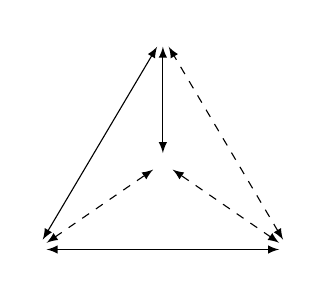
\begin{tikzpicture}
\node (re) at (0,0) {\RE};
\node (dfa) at (0,1.6) {\DFA};
\node (nfa) at (-1.6,-1.1) {\NFA};
\node (enfa) at (1.6,-1.1) {\ENFA};

\draw[latex-latex] (dfa) -- (nfa);
\draw[latex-latex] (nfa) -- (enfa);
\draw[latex-latex, dashed] (enfa) -- (dfa);
\draw[latex-latex] (dfa) -- (re);
\draw[latex-latex, dashed] (nfa) -- (re);
\draw[latex-latex, dashed] (enfa) -- (re);
\end{tikzpicture}
\end{center}
In our diagram, a solid line indicates that we have a method of directly converting between two models of computation, while a dashed line indicates that we have an indirect method---say, by performing two consecutive conversion steps.

All of our conversions considered apart may seem like nothing more than mechanical procedures or unimportant intermediate steps that we can employ in some larger system. However, taken together as we did in our diagram, these conversions reveal what might reasonably be called the most important theorem in the entire study of regular languages.

\begin{theorem}[Kleene's theorem]\label{thm:kleene}
A language $R$ is regular if it satisfies any of the following equivalent properties:
\begin{enumerate}
\item There exists a deterministic finite automaton $\mathcal{M}_{\text{D}}$ such that $L(\mathcal{M}_{\text{D}}) = R$;
\item There exists a nondeterministic finite automaton $\mathcal{M}_{\text{N}}$ such that $L(\mathcal{M}_{\text{N}}) = R$;
\item There exists a nondeterministic finite automaton with epsilon transitions $\mathcal{M}_{\text{E}}$ such that $L(\mathcal{M}_{\text{E}}) = R$; or
\item There exists a regular expression \regex{r} such that $L(\regex{r}) = R$.
\end{enumerate}
\end{theorem}

Note that we don't need to prove anything here---the proof of Kleene's theorem is baked into the descriptions of each of our conversion procedures!